\documentclass{article}
\usepackage{import}
\usepackage{graphicx}
\usepackage[utf8]{inputenc}
\usepackage[english]{babel}
\usepackage{amsmath}
\usepackage{biblatex}
\bibliography{ref.bib}

\title{ETERNITY: NUMBERS - Silver Ratio $(\delta_s)$}
\author{Md Hasibul Huq}
\date{July 2019}

\begin{document}               % plus the \end{document} command at the end.
\maketitle

\section{Introduction}          % This command makes a section title.

This document provides an understanding of only an irrational  number called Silver Ratio $(\delta_s)$. An irrational  number is  not  a rational  number, it is not possible to express an irrational number as a quotient of two integers.
\subsection{History}
Silver Ratio is studied from the time of Greek knowledge, which discusses the fundamental characteristics of the number system. Though it is not used by normal people intentionally. Silver ratio is the limiting of consecutive  of infinite sequence of integers, The silver ratio is presented in a Greek symbol ($\delta_s$).

\subsection{Mathematical Definition}
The value of silver ration is 2.4142135623 \cite{jdc_silver}. A ratio of the sequential sum of smaller number and twice of the larger number, which will produce an infinite sequence and the ration between smaller and larger number will be always same \cite{numberphile_silver}. This can be presented in mathematical equation:- 

\[ \dfrac{2a + b}{a}  = \dfrac{b}{a} = \delta_s \] \newline

It will be easier to understand if it can be compared with Fibonacci number.
In Fibonacci, the smaller and larger number are added to get the next one. 
Example:-

\[1,1,2,3,5,8,13,..\] \newline

For silver ratio, the smaller and twice of the larger number are added to get the next one. Example:-

\[1,2,5,12,29,70,..\] 

Then the latest number is divided  by the previous larger number. 

\import{./}{interview.tex}

\section{Persona}
\begin{figure}[h!]
  
  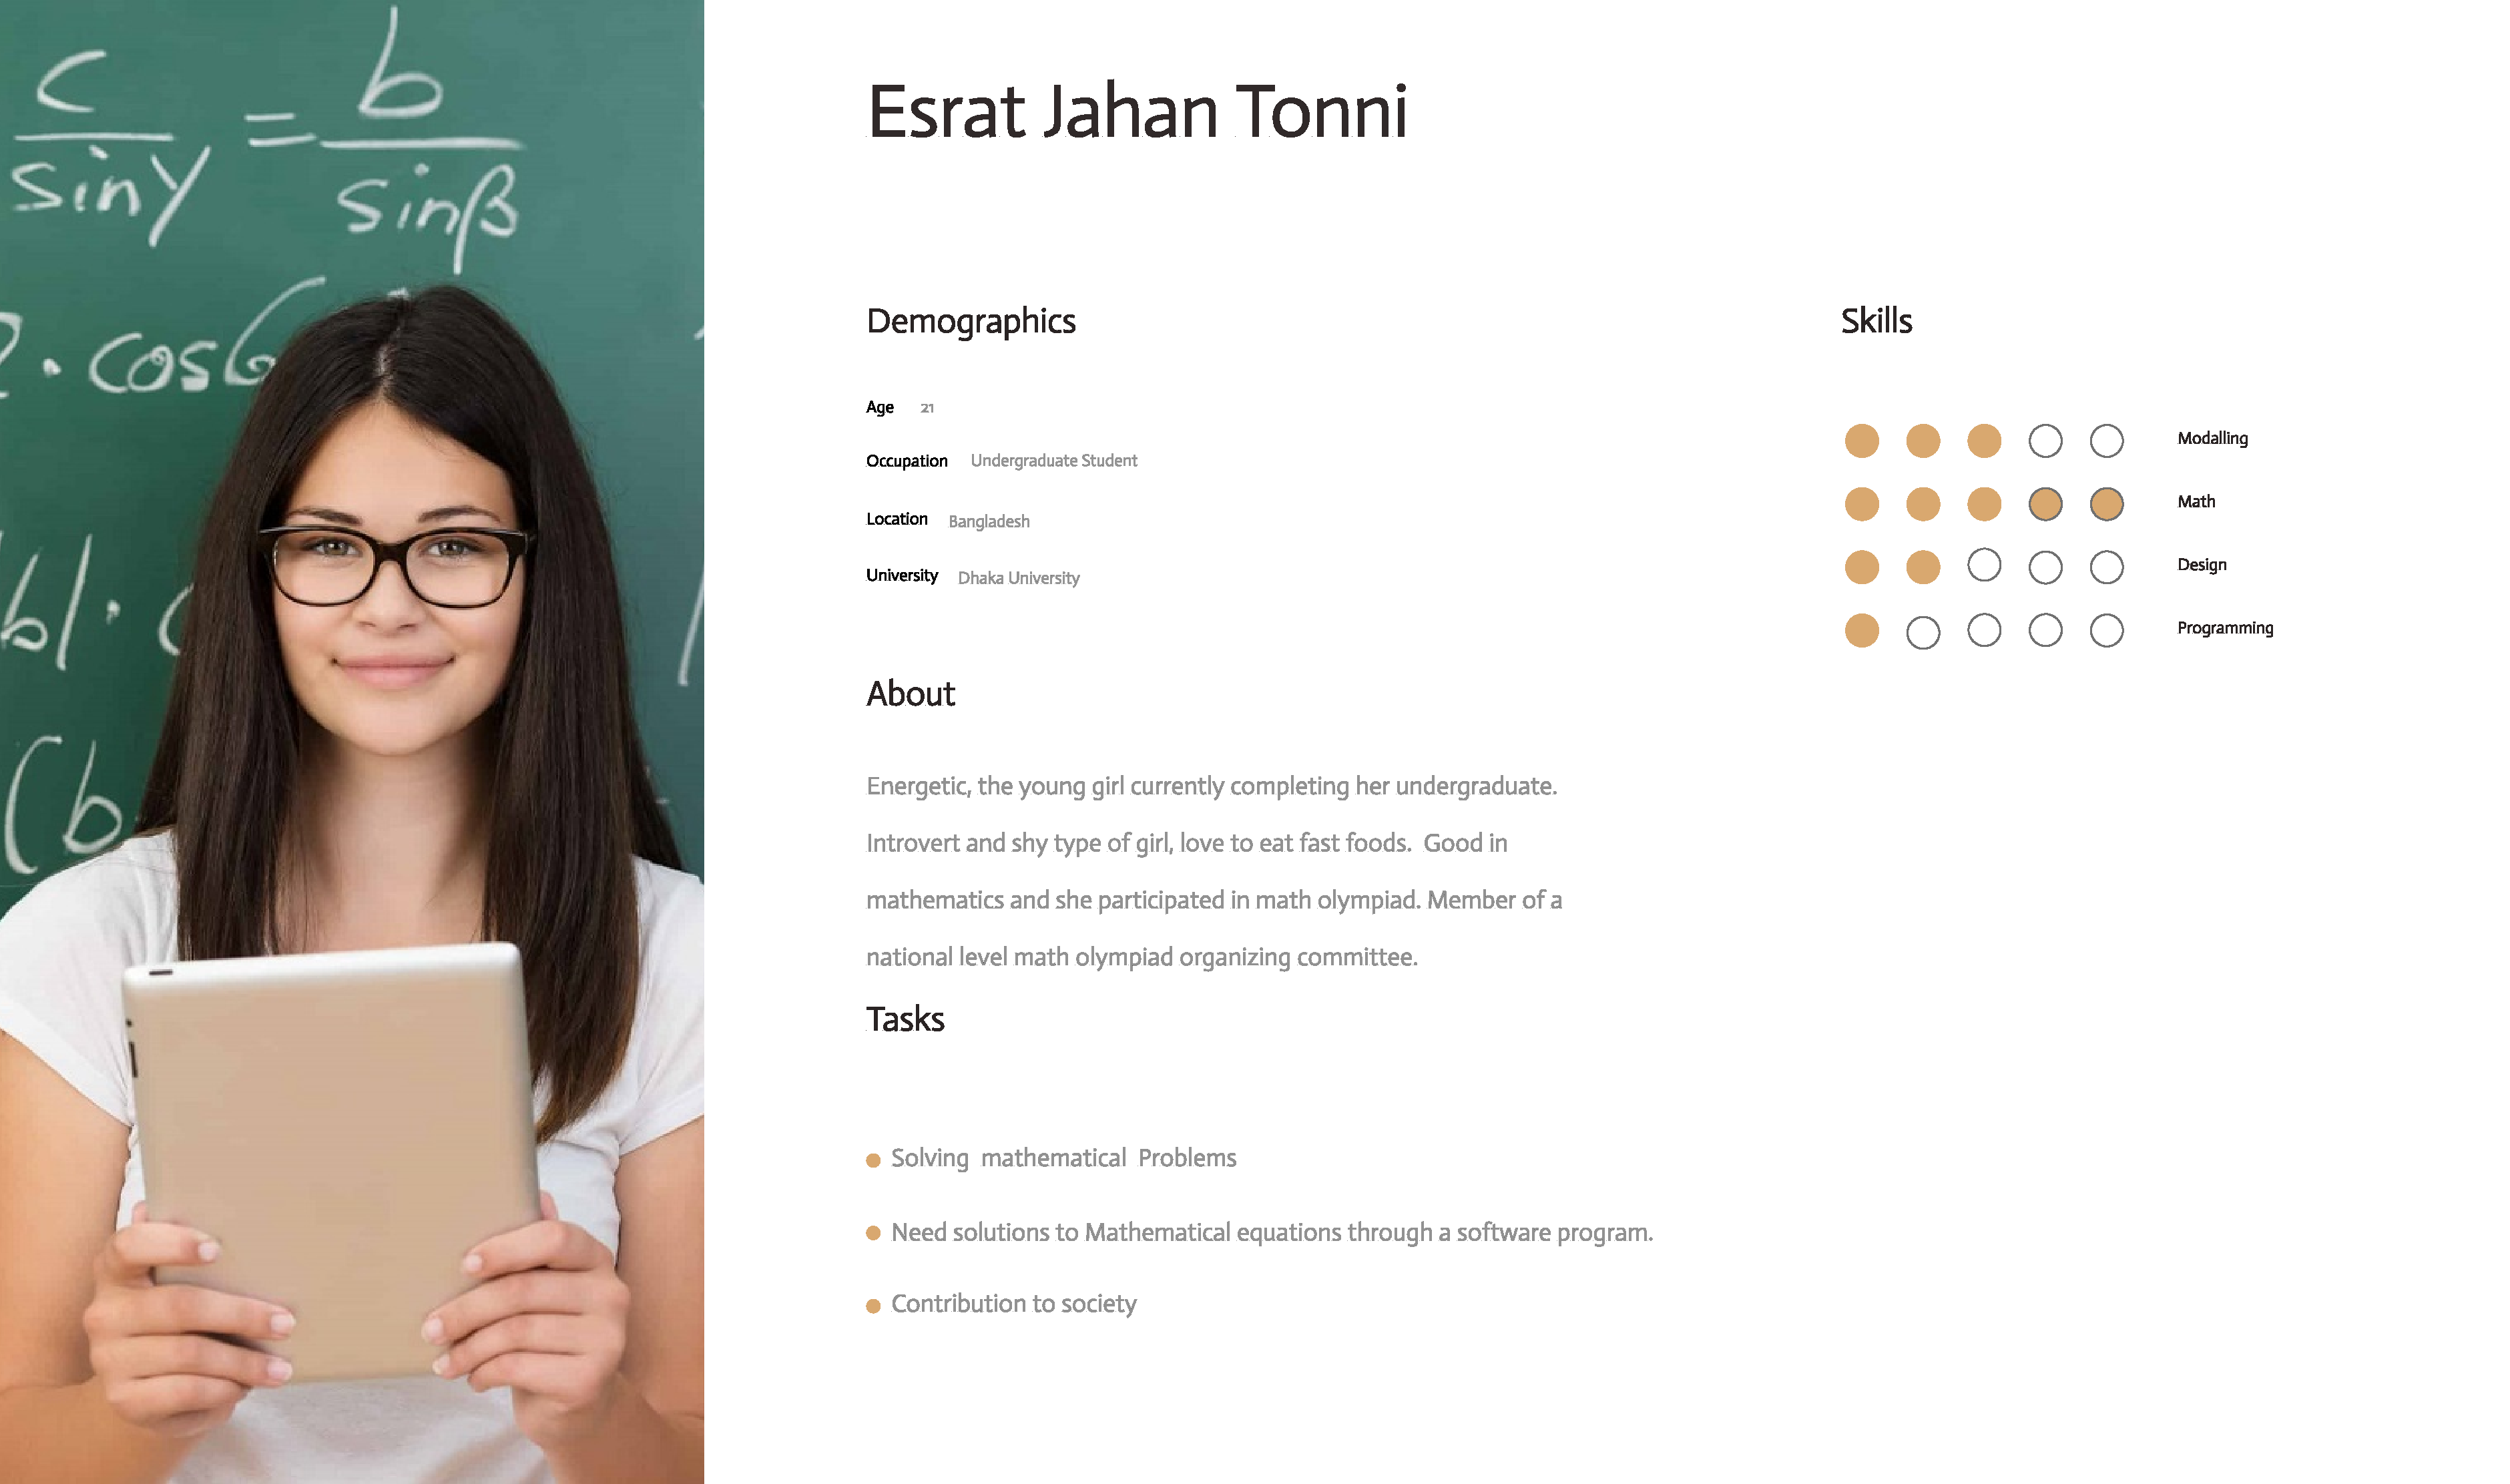
\includegraphics[width=1\textwidth]{persona}
  \centering
  \caption{Persona based on the analysis of interview
}
\end{figure}

\printbibliography

\end{document}                 % The input file ends with this command.
